\chapter{Aplicação 1: Câncer Labial na Escócia}\label{chap:lip}

\cite{Clayton1987} apresentam dados de casos registrados durante 6 anos (1975-1980) de câncer labial na Escócia.
Para cada um dos 56 condados da Escócia, temos como informação a contagem de casos observados, assim como o "valor esperado" de casos naquela região.
Este valor esperado é obtido através de características demográficas e foram calculados de acordo com \cite{Mantel1968} e aqui são tratados como constantes dadas. 

Ao invés de mapear os casos de câncer, mapeio a SIR (Standard Infection Ratio) em porcentagem para cada condado.
A SIR é dada por:

\begin{equation}
    \label{eq: SIR}
    SIR_i = 100 \times \frac{y_i}{E_i}, \quad i=1,\dots,n
\end{equation}
onde $y_i$ é o número de casos observados e $E_i$ é o valor esperado de casos para o condado $i$. Temos também como covariável a porcentagem a população envolvida em atividades de agricultura, caça e pesca por condado. Ambas as informações estão mapeadas pelas \autoref{fig:SIR Lip cancer} e \autoref{fig:AFF Lip cancer}.
\begin{figure}[b]
\centering
\begin{minipage}{.45\textwidth}
  \centering
  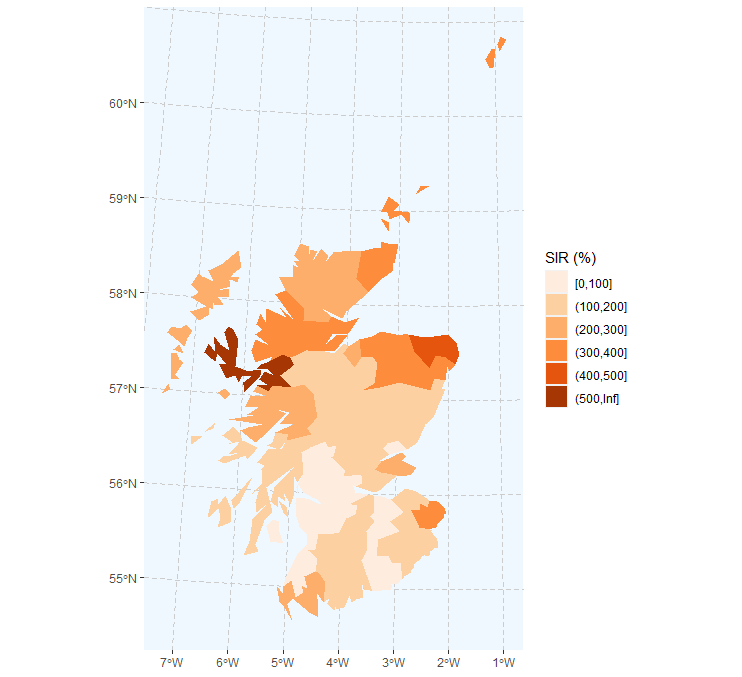
\includegraphics[width=\linewidth]{images/SIR_map_LIP.png}
  \captionof{figure}{Mapa da SIR em porcentagem para os condados da Escócia.}
  \label{fig:SIR Lip cancer}
\end{minipage}%
\begin{minipage}{.45\textwidth}
  \centering
  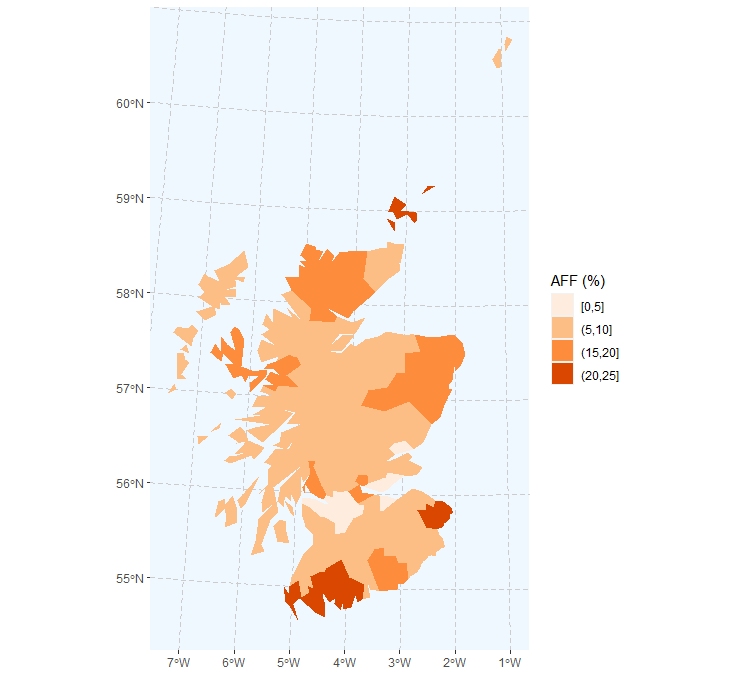
\includegraphics[width=\linewidth]{images/AFF_map_LIP.png}
  \captionof{figure}{Mapa da porcentagem da população envolvida em atividades de agricultura, caça e pesca (AFF).}
  \label{fig:AFF Lip cancer}
\end{minipage}
\end{figure}


Modelo o risco relativo $\theta_i$ em cada condado como

\begin{equation}
    \log(\theta_i) = \beta_0 + \beta_1 \cdot AFF_i + \xi_i,
\end{equation}

onde $\beta_1$ é o efeito da covariável $AFF$ e $\xi_i$ termo de erro para capturar a sobre-dispersão da Poisson. Serão usadas 4 formulações para $\xi_i$ revisadas no Capítulo 2: erro não-estruturado, termo CAR, o modelo de BYM e o modelo BYM2. As simulações da posteriori são feitas utilizando Cadeias de Markov e Monte Carlo. A linguagem utilizada foi R na versão 4.1.3. Para rodar as cadeias, a biblioteca Nimble, versão 0.12.2 e em especial para o calculo do fator de escala do BYM2 o pacote INLA versão 22.05.03. Todas as cadeias foram rodadas para um número fixo de 10.000 iterações com 2.000 iterações de \textit{burn-in}, 4 cadeias em paralelo para cada modelo. Todas as cadeias apresentaram no diagnóstico de Gelman-Rubin  $\hat{R} < 1.05$.\\

Para todos os modelos foram escolhidas prioris vagas  para $\beta_0$ e $\beta_1$, normais de média zero e precisão $10^{-3}$. Todos os modelos também seguem a recomendação de \cite{Sterrantino2018} para modelar casos onde existem ilhas desconectadas (no caso da Escócia, existem 3 ilhas), e modelam a taxa relativa nas ilhas sem componente estruturada.

Os parâmetros de precisão para serem calibrados são $\tau_s$, $\tau_u$ e $\tau_r$, precisão da componente estruturada, precisão da componente não estruturada e precisão conjunta, respectivamente. Seguindo a mesma prática que \cite{Wakefield2007}, atribuo prioris $Gamma(1,0.1)$ para esses parâmetros. Para o parâmetro de mistura $\rho$ do BYM2, a priori não-informativa $Beta(1,1)$. A \autoref{tab:posterior_summary_scotland} mostra o sumário da mediana à posteriori junto com intervalos de credibilidade inferiores e superiores para o intercepto e o coeficiente a covariável AFF. O WAIC de cada modelo também é exibido na tabela. Note que entre os modelos que possuem componente espacial, quase não há diferença entre as estimativas dos parâmetros. A principal diferença entre eles é a interpretabilidade de cada hiperparâmetro, como nota também \cite{Ribler2019}. 

\begin{table}

\centering
\begin{tabular}{@{}lrrcrrcc@{}}\toprule
& \multicolumn{2}{c}{$\beta_0$} & \phantom{ab}& \multicolumn{2}{c}{$\beta_1$}&\phantom{ab}& WAIC\\

%\cmidrule{2-3} \cmidrule{5-6}
%& $Média$ & $(upp,lwr)$ && $Média$ & $(upp,lwr)$\\
\midrule
\textbf{Poisson lognormal} & -0.49 & (-0.80,-0.19) && 6.88 & (3.97, 9.64) && 307.7\\  % var.u 0.59 (0.45 0.78)
\textbf{CAR} & -0.31 & (-0.55, -0.08) && 4.38 & (1.84, 6.82) && 300.2\\ 
% var.s  0.6504600  0.6433667 0.1170732  0.4446273  0.90150079
\textbf{BYM} & -0.33 & (-0.59, -0.07) && 4.94 & (2.22, 7.50) && 303.3\\ 
%var.r  0.4729313  0.4660862 0.0755433  0.3424083  0.64046237
\textbf{BYM2} & -0.32 & (-0.57, -0.06) && 4.60 & (1.74, 7.17) && 298.8\\
\bottomrule
\end{tabular}
    \caption{Sumários à posteriori para os modelos de Câncer Labial na Escócia. Para os parâmetros beta a média a posteriori junto com os intervalos de credibilidade superiores e inferiores de 95\%.}
    \label{tab:posterior_summary_scotland}
\end{table}

Para cada modelo temos também a SIR à posteriori como mostra a \autoref{fig7}. Observe como a componente espacial suaviza o mapa de risco da doença. Além disso, usando o teste de Moran no resíduo destes modelos, obtive O I de Moran com valor 0.21, contra um esperado de -0.019 (p-valor 0.006), alto indício de dependência espacial no resíduo. Já no modelo de BYM a estatística de Moran cai para -0.004 (p-valor de 0.86), ou seja, evidenciando uma diminuição da dependência espacial do resíduo, o que melhora a interpretação dos parâmetros do modelo \cite{Wakefield2007}.

Vale notar o parâmetro $\rho$ do modelo BYM2, que controla a mistura entre erro estruturado e não estruturado. A priori supuz indiferença para este parâmetro, e comecei as cadeias com valores de $\rho$ diferentes, variando a contribuição de cada tipo de erro. A posteriori converge para uma concentração maior de erro estruturado. A mediana à posteriori de $\rho$ foi $0.83 (0.36,0.99)$, o que pode explicar o Modelo de Besag ter tido um WAIC menor (afinal, ele possui erro estruturado puro). A vantagem do BYM2 é poder agora analisar o parâmetro $\tau_r$ e entender quanto da SIR à posteriori foi explicada pelo erro. Lembrando que o erro tem média constante zero, a mediana do desvio padrão à posteriori vale $0.47 (0.34, 0.64)$. 
\begin{figure}[ht] 
  \begin{subfigure}[b]{0.5\linewidth}
    \centering
    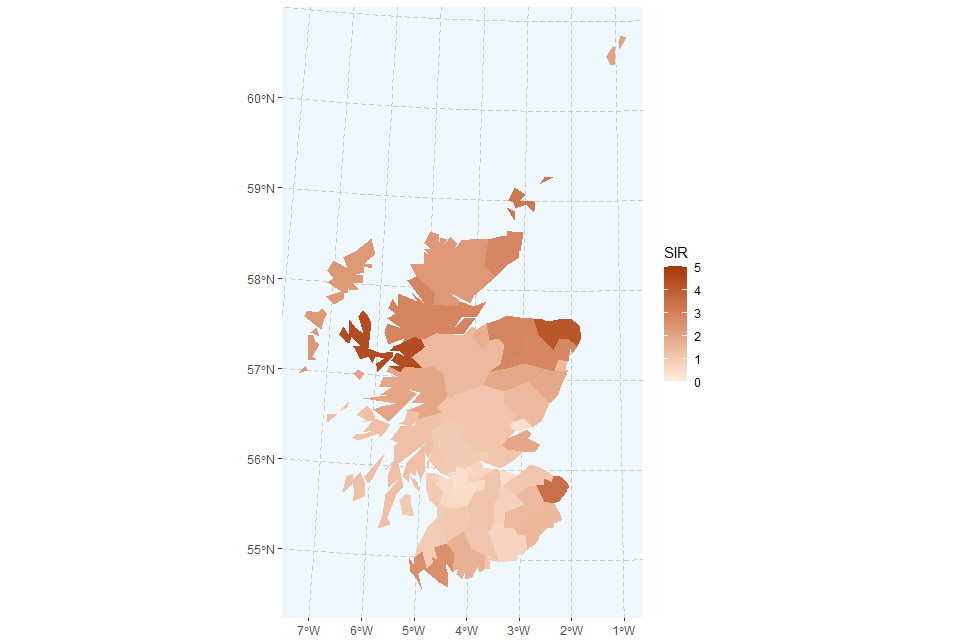
\includegraphics[width=0.9\linewidth]{images/SIR_posteriori_noCAR.png} 
    \caption{Modelo Poisson log-normal puro} 
    \label{fig7:a} 
    \vspace{4ex}
  \end{subfigure}%% 
  \begin{subfigure}[b]{0.5\linewidth}
    \centering
    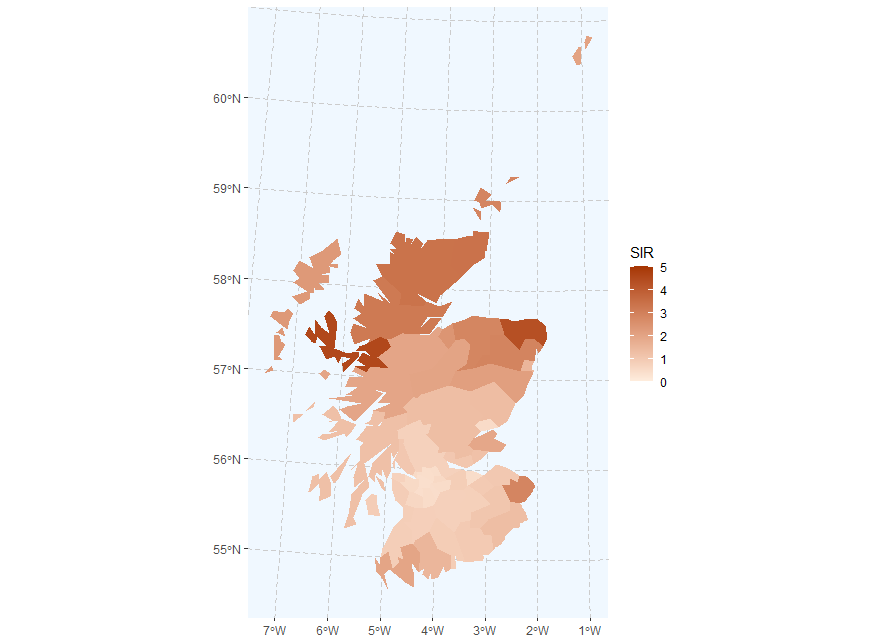
\includegraphics[width=0.9\linewidth]{images/SIR_posteriori_CAR.png} 
    \caption{Modelo de Besag} 
    \label{fig7:b} 
    \vspace{4ex}
  \end{subfigure} 
  \begin{subfigure}[b]{0.5\linewidth}
    \centering
    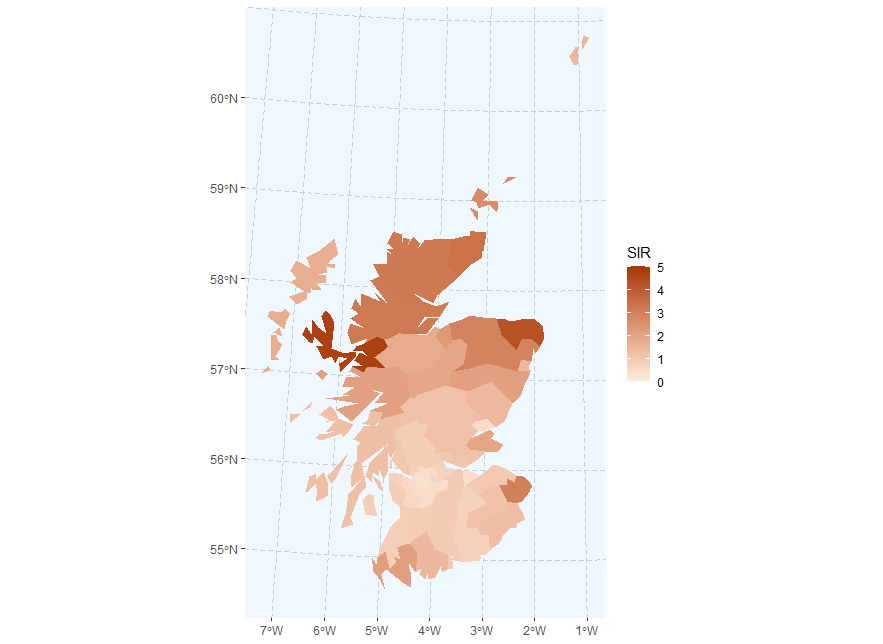
\includegraphics[width=0.9\linewidth]{images/SIR_posteriori_BYM.png} 
    \caption{Modelo BYM} 
    \label{fig7:c} 
  \end{subfigure}%%
  \begin{subfigure}[b]{0.5\linewidth}
    \centering
    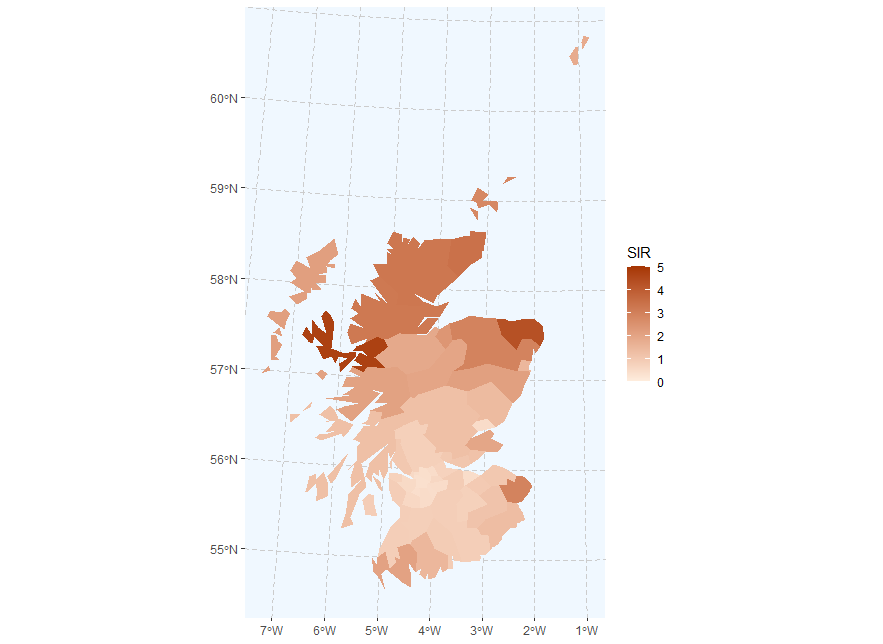
\includegraphics[width=0.9\linewidth]{images/SIR_posteriori_BYM2.png} 
    \caption{Modelo BYM2} 
    \label{fig7:d} 
  \end{subfigure} 
  \caption{SIR à posteriori média para cada um dos modelos analisados. Observe como o modelo sem componente espacial possui o mapa da SIR bem similar ao da taxa crua, e como os modelos espaciais distribuem o efeito da doença para as vizinhanças, promovendo suavização.}
  \label{fig7} 
\end{figure}


Uma última análise interessante é verificar a probabilidade à posteriori da SIR em um determinado condado ser maior que 1. A figura trás essa visualizacão para o modelo BYM2.

\begin{figure}[h]
    \centering
    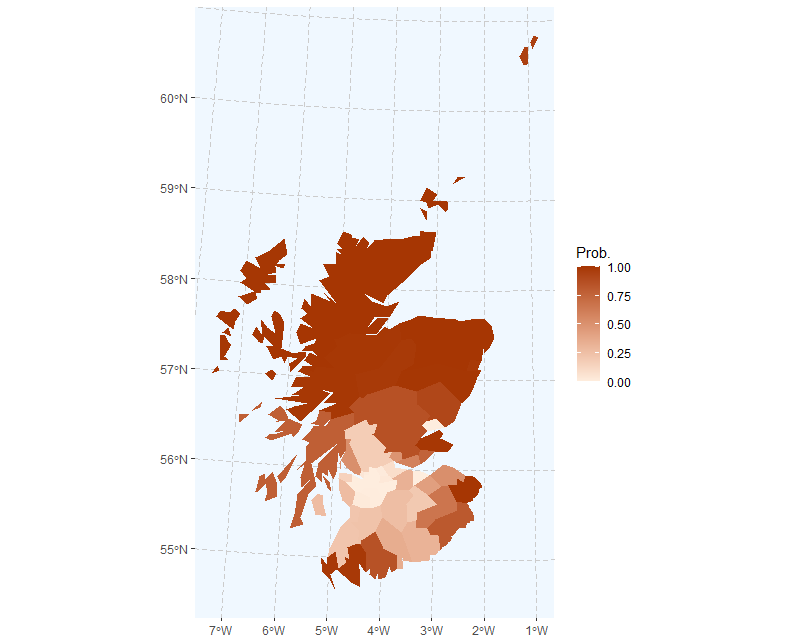
\includegraphics[width = 0.8\linewidth]{images/prob_greater_1.png}
    \caption{Probabilidade à posteriori da SIR ser maior que 1 (modelo BYM2)}
    \label{fig:my_label}
\end{figure}
